One ring to rule them all -- see the ring in Figure \ref{fig:ring}

One by one, the free lands of Middle-Earth fell to the power of the Ring, but there were some who resisted. A last alliance of men and elves marched against the armies of Mordor, and on the very slopes of Mount Doom, they fought for the freedom of Middle-Earth. Victory was near, but the power of the ring could not be undone. It was in this moment, when all hope had faded, that Isildur, son of the king, took up his father’s sword.


\begin{figure}
    \centering
    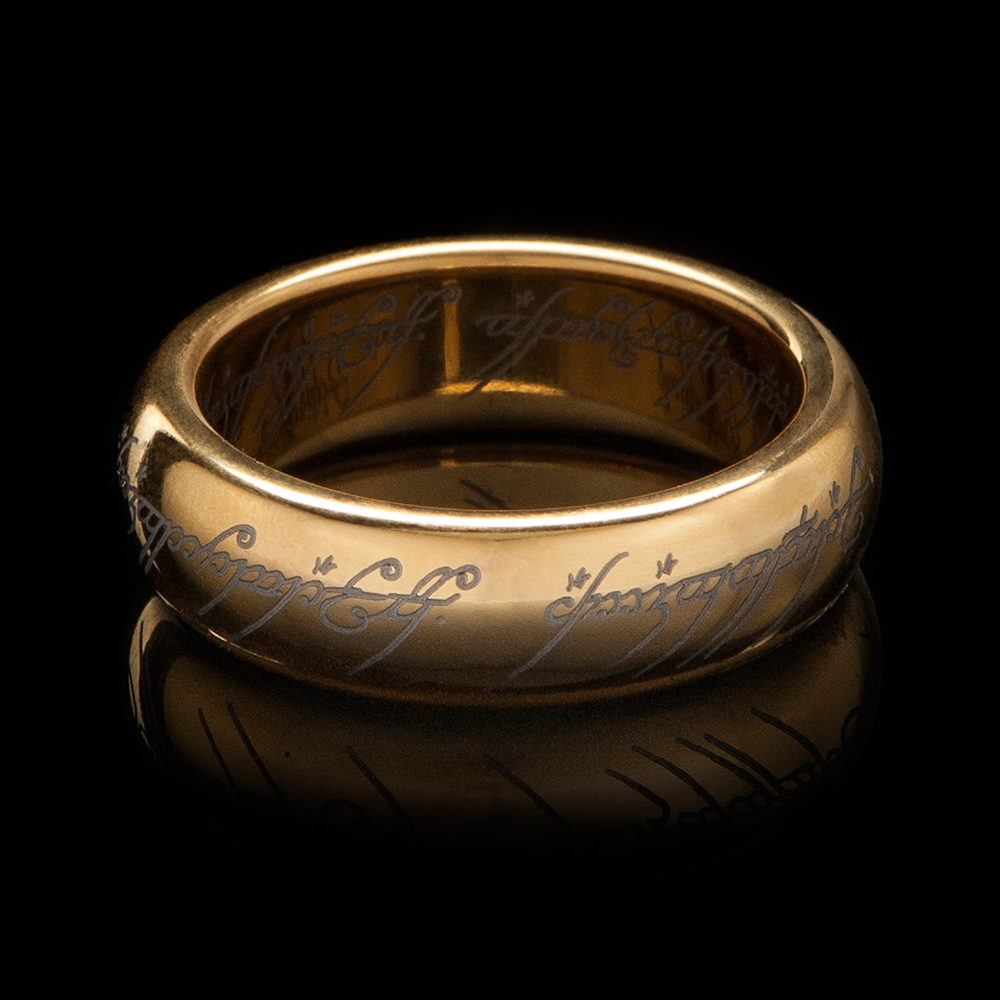
\includegraphics[width=0.5\textwidth]{src/imgs/ring.jpg}
    \caption{An illustration of the powerful ring}
    \label{fig:ring}
\end{figure}


Sauron, enemy of the free peoples of Middle-Earth, was defeated. The Ring passed to Isildur, who had this one chance to destroy evil forever, but the hearts of men are easily corrupted. And the ring of power has a will of its own. It betrayed Isildur, to his death.

And some things that should not have been forgotten were lost. History became legend. Legend became myth. And for two and a half thousand years, the ring passed out of all knowledge. Until, when chance came, it ensnared another bearer \cite{tolkien2012fellowship}.

It came to the creature Gollum, who took it deep into the tunnels of the Misty Mountains. And there it consumed him. The ring gave to Gollum unnatural long life. For five hundred years it poisoned his mind, and in the gloom of Gollum’s cave, it waited. Darkness crept back into the forests of the world. Rumor grew of a shadow in the East, whispers of a nameless fear, and the Ring of Power perceived its time had come. It abandoned Gollum, but then something happened that the Ring did not intend. It was picked up by the most unlikely creature imaginable: a hobbit, Bilbo Baggins, of the Shire.

For the time will soon come when hobbits will shape the fortunes of all.